\chapter{Jogos Evolucionários em Redes Finitas}

\begin{figure}[h]
    \caption{As diferentes estruturas populacionas em jogos. (a) População mista (jogadores atômicos com estratégias diferentes são representados por formas diferentes). (b) Grupos de jogadores atômicos com traços diferentes agrupados em subpopulações. (c) Subpopulações representadas como vértices em um grafo completo. (d) Subpopulações representadas como vértices de um grafo genérico. Imagem retirada de \cite{madeo2015}.}
    \centerline{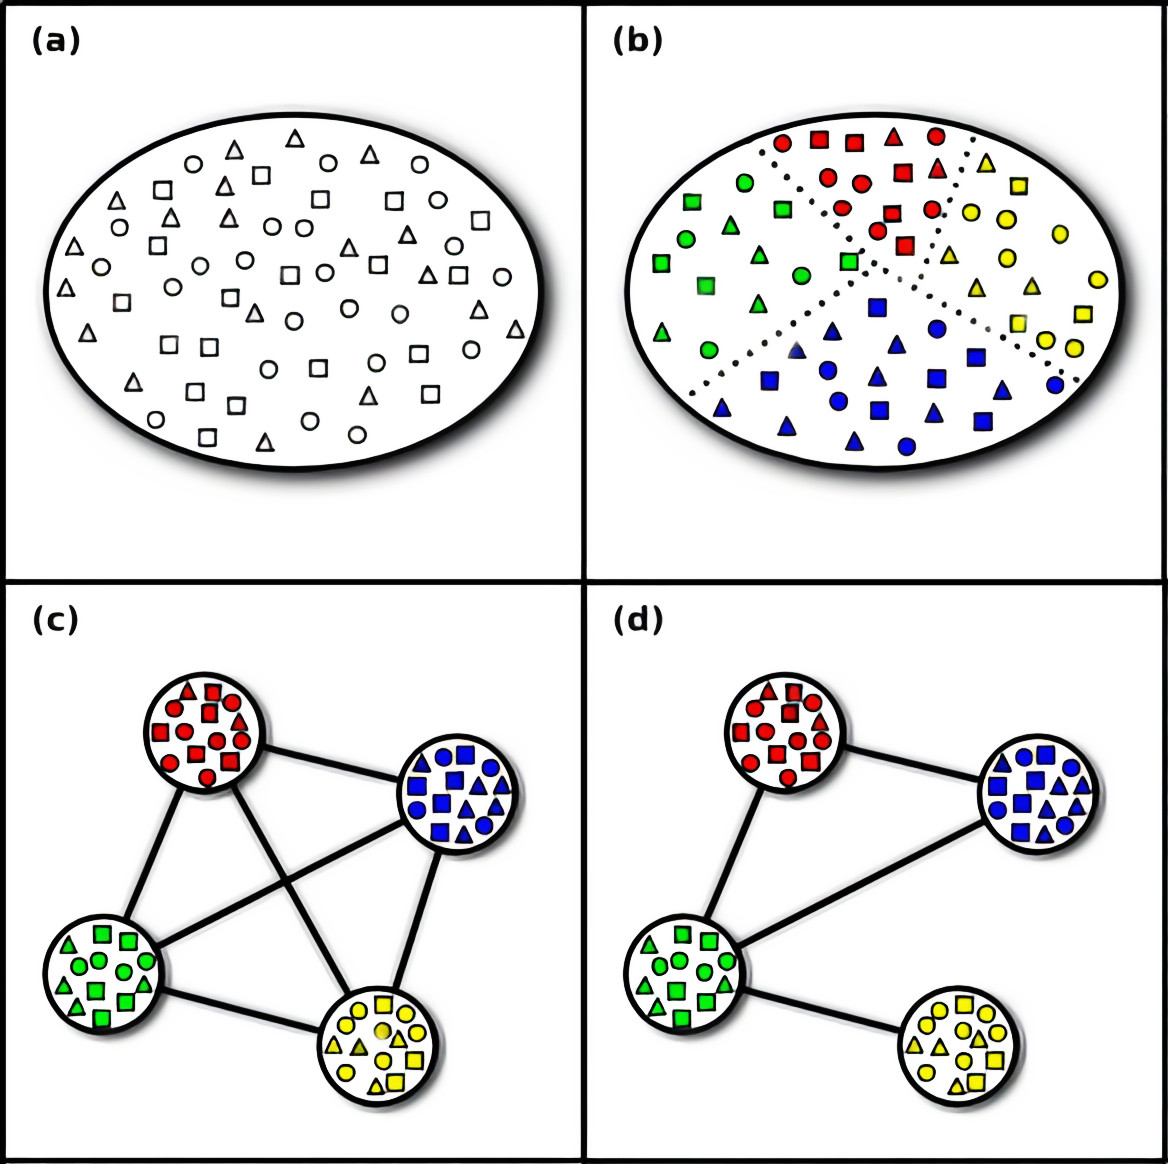
\includegraphics[scale=0.22]{./img/dif_populacao.jpg}}
    \label{fig:dif_populacao}
\end{figure}

Em situações reais, interações entre um número finito de indivíduos podem estar sujeitas a restrições topológicas, na qual jogadores irão interagir somente com um número reduzido de indivíduos próximos de acordo com essa topologia. Nesse contexto, Madeo e Mocenni \cite{madeo2015} introduziram um modelo que estende a teoria dos jogos evolucionários para redes finitas, representadas por grafos que descrevem as conexões entre os jogadores. Grafos são estruturas formadas por vértices e arestas, que são pares de vértices, e são usados para descrever os mais variados tipos de redes. Iremos considerar cada subpopulação como um jogador vértice, que usa a estratégia mista corresponde à distribuição de estratégias puras da subpopulação. Podemos ver abaixo na figura \ref{fig:dif_populacao}(c) um jogo em rede equivalente ao jogo multipopulação em \ref{fig:dif_populacao}(b), descrito através de um grafo completo, onde todos vértices estão conectados entre si.

Na figura \ref{fig:dif_populacao}(d) temos um jogo em redes finitas, onde nem todos jogadores vértices estão conectados devido às restrições topológicas. Uma aresta entre dois jogadores indica que eles interagem, porém um jogador pode considerar alguma interação como mais importante que as outras e dois jogadores podem ter percepções diferentes sobre a importância daquela interação e, até mesmo, a interação ser unilateral. Portanto, os grafos serão, em geral, direcionados e ponderados, onde um peso positivo na aresta indica a importância dada pelo jogador de origem para aquela interação.

Formalmente, seja $\G$ um grafo direcionado e ponderado com $N<\infty$ vértices (de ordem $N$) e $\V=\{1,2,\dots,N\}$ o seu conjunto de vértices. O grafo $\G$ é completamente descrito por sua matriz de adjacências $A\in\R^{N\times N}_{\geq0}$. Mais precisamente, sempre que há uma aresta que sai do jogador $v$ e termina no jogador $u$ a entrada $a_{v,u}$ da matriz será o peso que $v$ dá para a interação com $u$. Quando $a_{v,u}>0$ e $a_{u,v}=0$, somente $v$ receberá um pagamento na interação com $u$. Por fim, se $a_{v,u}=a_{u,v}=0$ quer dizer que $v$ e $u$ não interagem entre si. Além disso, nesse modelo assumimos que não existem loops, ou seja, arestas que saem de $v$ e terminam em $v$. Em outras palavras, temos $a_{v,v}=0, \forall v\in\V$.

A seguir iremos definir o pagamento e a equação de replicação para jogos evolucionários em redes finitas e listar algumas propriedades e definições importantes para o trabalho.

% -- % -- % -- %

\section{Pagamento e Equilíbrio de Nash em Redes Finitas}

A cada instante dois jogadores vértices que estão conectados são selecionados para jogar entre si. Um replicador de cada vértice é escolhido aleatoriamente para o jogo e o pagamento é o sucesso reprodutivo, de maneira análoga aos jogos multipopulação que vimos até o momento. Assim, o pagamento esperado de um jogador vértice depende das interações com todos os jogadores com os quais ele está conectado, a sua vizinhança. Dado um perfil de estratégias $\BS{X}\in\Delta$, podemos definir o pagamento esperado de $v\in\V$ como
\begin{equation}
    \label{pagtoWS}
    \pi^\G_v(\BS{X})= \BS{x_v} B_v \BS{k_v}(\BS{X})
\end{equation}
onde $B_v$ é a matriz de pagamentos de $v$ para o jogo e $\BS{k_v}(\BS{X})=\frac{1}{d_v}\sum^N_{u=1} a_{v,u} \BS{x_u}$, com $d_v=\sum^N_{u=1} a_{v,u}$, o grau do vértice $v$. Note que o pagamento esperado nada mais é que a soma do pagamento de todas interações dois à dois ponderada pelo peso das arestas do grafo. Para simplificar a notação, defina o pagamento esperado de $v$ ao usar a estratégia pura $s\in S$ por $p^\G_{v,s}=\pi^\G_v(\BS{e_s},\BS{X_{-v}})$ e o pagamento esperado de $v$ ao usar a estratégia mista $\BS{x_v}\in\Delta_M$ por $\phi^\G_v=\pi^\G_v(\BS{x_v},\BS{X_{-v}})$. 

Perceba que a estrutura do grafo está embutida na função de pagamentos e, portanto, a definição de equilíbrio de Nash é equivalente à definição \ref{DefEqNashClassico}, porém também pode ser definido em função do pagamento esperado para estratégias puras da seguinte maneira.

\begin{definition}
    \label{defEqNashEstPura}
    O conjunto de equilíbrio de Nash é definido como sendo
    \begin{equation*}
        \Theta^{NE}=\{\BS{X}\in\Delta\;\mid\;  \forall v,\forall x_{v,s}>0, p^\G_{v,s}=p^\G_{v,s'}, \forall x_{v,s'}>0 \;\;\text{e}\;\; p^\G_{v,s}\geq p^\G_{v,s'}, \forall x_{v,s'}=0\}
    \end{equation*}
    E o conjunto de equilíbrio de Nash estrito é dado por
    \begin{equation*}
        \Theta^{NES}=\{\BS{X}\in\Delta\;\mid\;  \forall v,\forall x_{v,s}>0, p^\G_{v,s}>p^\G_{v,s'}, \forall x_{v,s'}=0\}.
    \end{equation*}
\end{definition}

Em outras palavras, um perfil de estratégias é um equilíbrio de Nash se, para todo jogador, nenhuma das estratégias presentes no perfil possui vantagem sobre as demais e a aptidão das estratégias que não estão presentes no perfil é menor ou igual que a aptidão das demais. Novamente, equilíbrio é estrito se a desigualdade for estrita.

% -- % -- % -- %

\section{Equação de Replicação}

Usando a função de pagamento definida em $\eqref{pagtoWS}$ a equação de replicação multipopulação pode ser estendida para jogos em grafos \cite{madeo2015}, resultando no seguinte problema de Cauchy.

\begin{equation}
    \label{EqRepEGN}
    \left\{\begin{matrix*}[l]
        \dot{x}_{v,s}(t)=x_{v,s}(t)\left(\rho^\G_{v,s}(t)-\phi^\G_v(t)\right)\\
        x_{v,s}(0)=c_{v,s}
    \end{matrix*}\right.
    \;\;\forall v\in\V,s\in S
\end{equation}
onde $\BS{x_v}(0)=[c_{v,1}\dots c_{v,M}]\in\Delta_M$ é a condição inicial do jogador $v$.

A equação de replicação para jogos em grafos também é invariante em $\Delta$. Além disso, estratégias puras e equilíbrios de Nash são estados estacionários de $\eqref{EqRepEGN}$ e um perfil de estratégias $\BS{X^*}\in\text{int}(\Delta)$ é um estado estacionário se, e somente se, $\BS{X^*}\in\Theta^{NE}$.

O teorema a seguir mostra que a equação de replicação clássica pode ser obtida como um caso especial da equação de replicação em grafos. Para isso, mostraremos que as soluções da equação em grafos $\eqref{EqRepEGN}$ e da equação clássica $\eqref{eqRep}$ são equivalentes sob algumas hipóteses.

\begin{theorem}[Madeo e Mocenni \cite{madeo2015}]
    \label{TeoEquivalenciaEGN}
    Seja $\BS{X}(t)=\{\BS{x}_1(t)\dots\BS{x}_N(t)\}$ a única solução do problema de Cauchy $\eqref{EqRepEGN}$, onde $x_{v,s}(0)=c_s, \forall v$. Assuma também que $B_v=B, \forall v$. Seja $\BS{y}(t)$ a única solução do problema de Cauchy $\eqref{eqRep}$, com $y_s(0) = c_s$. Então, $\BS{x_v}(t)=\BS{y}(t), \forall v, \forall t\geq 0$.
\end{theorem}
\begin{proof}[Dem.:]
    Seja $\BS{X}(t)$ e $\BS{y}(t)$ como definido nas hipóteses. Tome um perfil de estratégias $\BS{Y}$ no qual a distribuição de estratégias de todos os $N$ jogadores é dada por $\BS{y}(t)$, a solução do problema $\eqref{eqRep}$. Com isso, temos
    \begin{equation*}
        \BS{k_v}(\BS{Y})=\frac{1}{d_v}\sum^N_{u=1}a_{v,u}\BS{y}(t)=\BS{y}(t)
    \end{equation*}
    ou seja, como todos usam a mesma estratégia $\BS{y}(t)$, a média ponderada de todas interações é, também, $\BS{y}(t)$. Assim, os pagamentos de todos jogadores serão dados por
    \begin{equation*}
    \begin{split}
        p^\G_{v,s}&=\BS{e_s}B\BS{k}_v(\BS{Y})=\BS{e_s}B\BS{y}=\pi_s\\
        \phi^\G_{v}&=\BS{x_v}B\BS{k}_v(\BS{Y})=\BS{y}B\BS{y}=\phi
    \end{split}
    \end{equation*}
    Logo, a equação de replicação em grafos aplicada ao perfil de estratégias $\BS{Y}$ é dada por
    \begin{equation*}
        \dot{y}_{v,s}=y_{v,s}(p^\G_{v,s}-\phi^\G_v)=y_s(\pi_s-\phi)=\dot{y}_s
    \end{equation*}
    Então, $\BS{Y}(t)$ é uma solução da equação $\eqref{EqRepEGN}$ e, pela unicidade da solução do problema de Cauchy $\eqref{EqRepEGN}$, temos que $\BS{x_v}(t)=\BS{y}(t),\forall v,\forall t\geq 0$. Em outras palavras, dados $\BS{X}(t)$ e $\BS{y}(t)$ como definido nas hipóteses, a equação de replicação em grafos é equivalente a equação de replicação clássica.
\end{proof}
